\documentclass{article}
\usepackage{titlesec}
\usepackage{verbatim}
%provides multi-line comment syntax : \begin{comment} \end{comment}
%provides href/url
\usepackage{hyperref}
\usepackage{cleveref}
\usepackage{xeCJK}
\usepackage[xetex]{graphicx}

\begin{comment}
\titleformat{\section}[runin]
  {\normalfont\Large\bfseries}{\thesection}{1em}{}
\titleformat{\subsection}[runin]
  {\normalfont\large\bfseries}{\thesubsection}{1em}{}
\titleformat{\subsubsection}[runin]
  {\normalfont\large\bfseries}{\thesubsection}{1em}{}
\end{comment}


\title{NASA hw4}
\author{B04902045 孫凡耘}
\date{\today}

\begin{document}
\maketitle
    \section{System Administration}
    \subsection{1}
    使用與lab相同的環境。\newline
    CentOS-7-x86\_64-Minimal-1611.iso\newline
    1. setup network with nmtui\newline
    2. yum install -y virt-install qemu-kvm libvirt\newline
    3. start and enable libvirt\newline
    \$ systemctl start libvirtd\newline
    \$ systemctl enable libvirtd\newline
    4. Download CentOS ISO\newline
    \$ curl [url] -o centos.iso\newline
    \$ mv centos.iso /var/lib/libvirt/images\newline
    \subsubsection{Task 1}
Enable "Virtualize Intel VT-x/EPT or AMD-V/RVI" in VM settings
\newline\newline
Verify Intel VT CPU virtualization extensions on a Linux\newline
Type the following command as root to verify that host cpu has support for Intel VT technology
\begin{verbatim}
$ grep --color vmx /proc/cpuinfo
\end{verbatim}
If the output has the vmx flags, then Intel CPU host is capable of running hardware virtualization.\newline
P.S. The /proc/cpuinfo file has information about the CPU.\newline
\newline
<方法一>\newline
You can specify a user which will have access to libvirt's setup (and thus creating VMs and pretty much running virsh commands) by adding the users to the libvirtd and kvm groups on the host.
\begin{verbatim}
$ sudo usermod -a -G libvirt <username>
$ sudo usermod -a -G kvm <username>
\end{verbatim}
Change group ownership and permissions on the default images directory:
\begin{verbatim}
$ sudo chown root:libvirt /var/lib/libvirt/images
$ sudo chmod g+rw /var/lib/libvirt/images
\end{verbatim}
after doing that, I was able to create VM with virt-install using non-root user, and only this certain user can create a VM without sudo.
\newline\newline

You can also use policykit to manage access, the procedure is described in the libvirt Wiki: \url{http://wiki.libvirt.org/page/SSHPolicyKitSetup}
\newline
Connect to VM host without root permission
\begin{verbatim}
virsh -c qemu+ssh://user@IP/system
user can be root or non-root user
\end{verbatim}



    \subsubsection{2}

\# for graphical console\newline

\begin{verbatim}
yum install virt-viewer

sudo virt-install -n VM_NAME --os-type=generic --ram=256 --vcpus=2 \
    --disk path=/dev/nasavg/lv1 \
    --graphics=vnc,password=MY_PASSWORD,listen=0.0.0.0,port=5903 \
    --location /var/lib/libvirt/images/centos.iso \
    --extra-args="ks=anaconda-ks.cfg console=tty0 console=ttyS0,115200n8" \
    --network bridge:virbr0

\end{verbatim}
    \newline
    parameters explained:\newline\newline
    \textbf{-n} NAME \newline
    \textbf{--os-type}=OS\_TYPE\newline
    \textbf{--ram}=MEMORY\newline
    \textbf{--vcpus}=Number of virtual processors to configure for the guest\newline
    \textbf{--disk path}=A path to some storage media to use\newline
    P.S. /dev/volume\_group/logical\_volume is the lvm of VM host\newline
    \textbf{--graphics=vnc,password=MY\_PASSWORD,listen=0.0.0.0,port=5903}\newline
    Set up a virtual console in the guest and export it as a VNC server in the host.\newline
    connect the VM to a VNC server listening on every interface (0.0.0.0) on port 5903 with password \newline
    \textbf{--location}\newline
    Specifies the installation source for guest virtual machine kernel+initrd pair(or ISO).\newline
    \textbf{--extra-args}=additional kernel command-line arguments to pass to the installer when performing a guest installation from a kernel+initrd.\newline
    \textbf{ks}=kickstart file path\newline
    P.S. I modified the kickstart file anaconda-ks.cfg\newline
    \textbf{--network}=NETWORK\newline
    The virbr0, or "Virtual Bridge 0" interface is used for NAT .\newline
    It is provided by the libvirt library, and virtual environments sometimes use it to connect to the outside network.\newline\newline
reference: \url{https://velenux.wordpress.com/2013/01/04/creating-a-new-libvirt-virtual-machine-from-the-command-line-with-virt-install/}
Problem encountered:
\begin{verbatim}failed to initialize KVM: Permission denied\end{verbatim}
Resolved by:
\begin{verbatim}
rmmod kvm_intel
rmmod kvm
modprobe kvm
modprobe kvm_intel
\end{verbatim}
\# Another way to use password to protect my vnc session
\begin{verbatim}
virsh edit centos
\end{verbatim}
Edit it as follow:
\begin{verbatim}
<graphics type='vnc' port='-1' autoport='yes' listen='192.168.1.5' \
passwd='PASSWORD-HERE' keymap='en-us'/>
\end{verbatim}
reference: \url{https://www.cyberciti.biz/faq/linux-kvm-vnc-for-guest-machine}

    \subsubsection{3}
    virsh console: Access a virtual machine's console over a serial connection\newline
    To do this on a physical machine, one has to do:\newline
    1. Configure console access on the target machine\newline
    2. On Linux: dterm, Minicom, picocom, Screen, Serialclient, For windows: gtkterm, Cutecom, putty\newline
    For detailed instructions: \url{https://wiki.archlinux.org/index.php/working_with_the_serial_console}
     \begin{figure}[!htb]
            \begin{flushleft}
            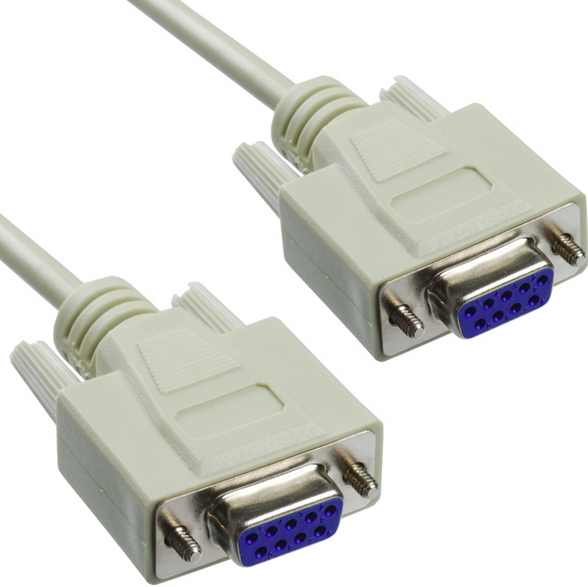
\includegraphics[scale=0.25]{screenshot.png}
            \end{flushleft}
    \end{figure}

    source: \url{http://keywordsuggest.org/gallery/762307.html}
    \newline P.S.\newline
    virsh ttyconsole <my VM name>\newline
    If the output is shown(mine is /dev/pts/0), it indicates the Guest has a console device already.


    \subsubsection{4}
1. Add console=ttyS0 to line in /boot/grub2/grub.cfg

should look something like this
\begin{verbatim}
linux16 /vmlinuz-3.10.0-123.el7.x86_64 \
root=UUID=ba0f2424-e66e-4862-90ff-7dccb63339c2 ro rd.lvm.lv=centos/swap \
vconsole.font=latarcyrheb-sun16 rd.lvm.lv=centos/root crashkernel=auto  \
vconsole.keymap=us LANG=en_US.UTF-8 console=ttyS0
\end{verbatim}
2. Allow login into ttyS0
\begin{verbatim}
$ echo "ttys0" >> /etc/securetty
\end{verbatim}
3. assert VM guest console type(should be serial)
\begin{verbatim}
<console type='pty' tty='/dev/pts/6'>
    <source path='/dev/pts/6'/>
    <target type='serial' port='0'/>
    <alias name='serial0'/>
</console>
\end{verbatim}
4. start ttyS0
\begin{verbatim}
$ sudo start ttyS0
or
$ systemctl enable serial-getty@ttyS0.service
$ systemctl start serial-getty@ttyS0.service
\end{verbatim}
5. login with
\begin{verbatim}
$ virsh console generic
\end{verbatim}
Above should do it but if you want to see even the grub2 menu options you can try the following:
in guest VM in /etc/default/grub replace
\begin{verbatim}
GRUB_CMDLINE_LINUX_DEFAULT="quiet"
#GRUB_TERMINAL=console
\end{verbatim}
by
\begin{verbatim}
GRUB_CMDLINE_LINUX_DEFAULT="console=tty0 console=ttyS0"
GRUB_TERMINAL="serial console"
\end{verbatim}
and
\begin{verbatim}
$ update-grub
\end{verbatim}
can login to your VM with the command virsh console
automatically after the vm boots.
reference: \url{http://blog.ls-al.com/kvm-virsh-console-on-centos-7/}\newline
reference: \url{https://mcdee.com.au/kvm-virsh-console-access-centos/}\newline
reference: \url{https://serverfault.com/questions/364895/virsh-vm-console-does-not-show-any-output}
    \subsubsection{5}


\textbf{Bridge to virbr0(NAT)}\newline
P.S.  Do *NOT* attempt to attach a physical device to 'virbr0' - this is only for NAT connectivity\newline
Execute the following command on VM host to bridge the VM to VM\_host through virbr0(NAT)
\begin{verbatim}
$ virsh attach-interface --domain generic --type bridge --source virbr0
\end{verbatim}
configure network with nmtui on VM guest(Activate the wired connection)\newline
reference: \url{https://kashyapc.fedorapeople.org/virt/add-network-card-in-guest.txt}\newline
\textbf{Bridging for VM}\newline
Use nmtui\newline
1. add a bridge connection named br0\newline
2. Add ens33 as slaves of br0\newline
3. reboot\newline
我們在這一步可以看到ens33下面的ip的設定了,br0下面有ip的設定\newline
4. execute the following command
\begin{verbatim}
$ virsh attach-interface --domain generic --type bridge --source br0
\end{verbatim}
5. Inside the vm of vm, dhclient the interface(attach之後跑出來的)
\begin{verbatim}
$ sudo dhclient ens9
\end{verbatim}
6. Done!\newline
這時可以看到vm host跟vm in vm有相同個網段,有gui那臺centos也可以ping到vm中的vm\newline
reference: \url{http://pominglee.blogspot.tw/2014/03/linux.html}
    \subsubsection{6}

1. virsh list\newline
2. virsh undefine VM\_NAME\newline
3. virsh domiflist VM\_NAME\newline
4. virsh detach-interface domain type\newline
5. virsh edit \newline

\end{document}
